\section{Motivation} \label{umfrage}

Zu Beginn wollten wir durch eine Meinungsumfrage überprüfen, ob bei Sprachassistenten mehr Datenschutz gewünscht ist. Dabei haben sich 110 Teilnehmer an der Umfragen beteiligt. Wir unterteilten die Teilnehmer in folgende Altersgruppen:

\begin{itemize}
	\item 0 bis 18 Jahre 
	\item 19 bis 25 Jahre
	\item 26 bis 35 Jahre
	\item 36 und älter	
\end{itemize}

\begin{figure}[h!]
	\centering
	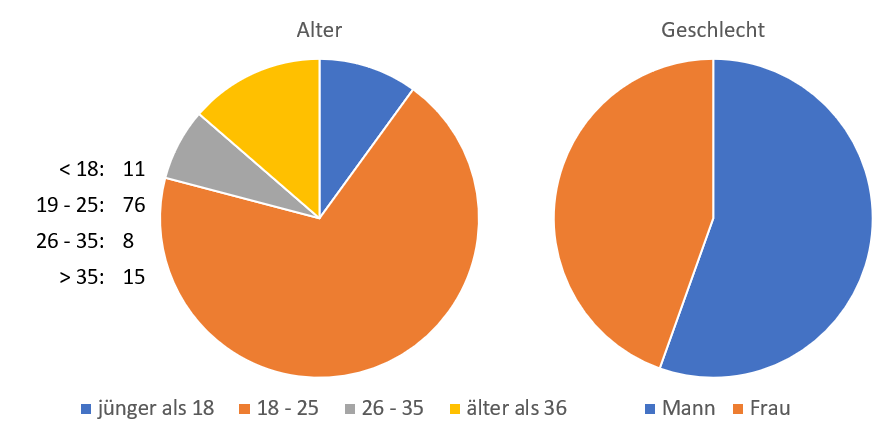
\includegraphics[width=0.7\linewidth]{Picture/umfrage_teilnehmer}
	\caption[Teilnehmer der Umfrage]{Teilnehmer der Umfrage}
	\label{fig:umfrage_teilnehmer}
\end{figure}

55,5 \% der Teilnehmer sind männlich und 45,5\% sind weiblich, wie in Abbildung \ref{fig:umfrage_teilnehmer} ersichtlich. Den Teilnehmern wurden folgende Fragen gestellt:

\begin{enumerate}
	
	\item Wie oft nutzen Sie ein Sprachassistent?
	\item Wissen Sie was mit Ihren Daten passiert?
	\item Würden Sie Geld für eine hohe Datensicherheit bezahlen?
	\item Wie viel Geld würden Sie für eine hohe Datensicherheit einer Anwendung bezahlen (einmalige Zahlung)?
	\item Bei welchen Anwendungen ist Ihnen Privatsphäre besonders wichtig?
	
\end{enumerate}

Bei der ersten Frage stellte sich heraus, dass mehr 54,5\% keine Sprachassistenten verwenden. Die bedeutet, dass 44,5\% einmal in Monat oder häufiger einen solchen Service in Anspruch nehmen. In den USA wurde eine Studie von highervisibility durchgeführt, bei der mehr als 70\% der Teilnehmer einen Sprachassistenten einmal im Monat oder häufiger verwenden\cite{highervisibility}.

\begin{figure}[h!]
	\centering
	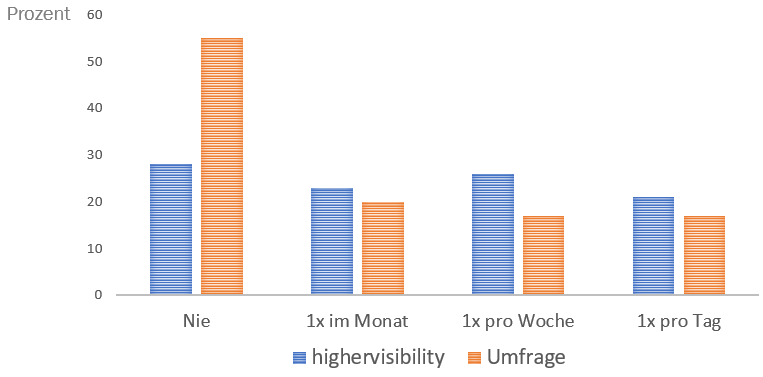
\includegraphics[width=0.7\linewidth]{Picture/umfrage_haeufigkeit}
	\caption[Nutzungshäufigkeit von Sprachassistenten]{Nutzungshäufigkeit von Sprachassistenten}
	\label{fig:umfrage_haeufigkeit}
\end{figure}

Bei den ausgewählten Testpersonen verwenden im Vergleich zur Umfrage, weniger Personen eine Sprachsteuerung. In Abbildung \ref{fig:umfrage_haeufigkeit} werden die Umfragen vergleichend illustriert. In den USA sind Menschen in verschiedenen Altersgruppe und regionaler Herkunft befragt worden. Die durchgeführte Umfrage hatte überwiegend junge Leute befragt. Erwartet wurde eine höhere Nutzung der Sprachsteuerung. 


Ungefähr 90\% der Teilnehmer haben angegeben, dass sie nicht wissen, was mit ihren Daten passiert, dass in Abbildung \ref{fig:umfrage_datenschutz} dargestellt ist. Die Zahlungsbereitschaft ist nach Altersgruppen in Abbildung \ref{fig:umfrage_geld_gruppen}  visualisiert. Jeder Vierte würde dabei für eine hohen Datensicherheit Geld bezahlen und 56\% der Teilnehmer sind sich unsicher, ob diese dafür Geld bezahlen würden. Die Altersbetrachtung nach der Zahlungsbereitschaft zeigt, dass die Gruppe unter 18 Jahren weniger bereit ist, Geld zu bezahlen. Die Schnittmenge der Teilnehmern, welche Ja oder vielleicht angekreuzt haben, steigt mit zunehmendem Alter.

\begin{figure}
	\centering
	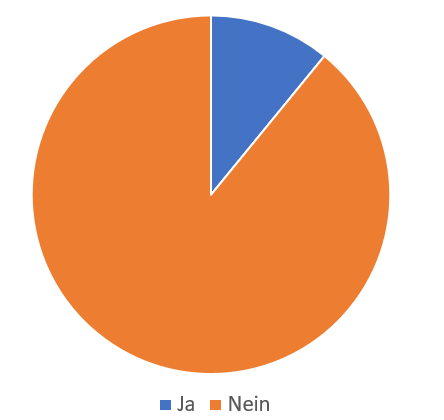
\includegraphics[width=0.5\linewidth]{Picture/umfrage_datenschutz}
	\caption[Relevanz des Datenschutzes für die Umfrageteilnehmer]{Relevanz des Datenschutzes für die Umfrageteilnehmer}
	\label{fig:umfrage_datenschutz}
\end{figure}



\begin{figure}[h!]
	\centering
	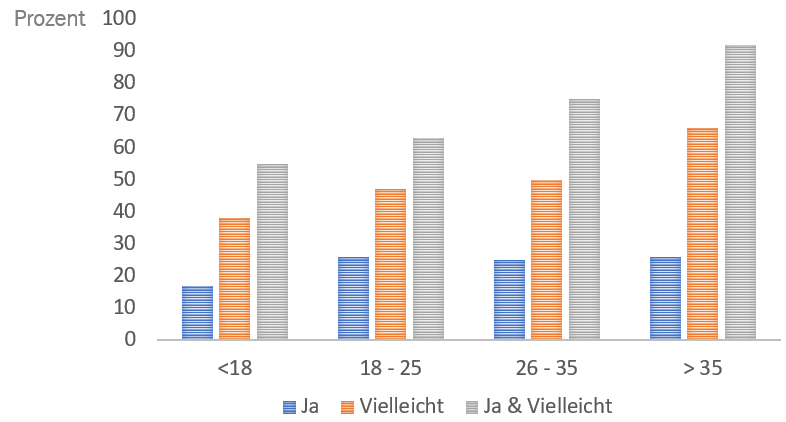
\includegraphics[width=0.7\linewidth]{Picture/umfrage_geld_gruppen}
	\caption[Zahlungsbereitschaft der Teilnehmer in verschiedenen Altersgruppen]{Zahlungsbereitschaft der Teilnehmer in verschiedenen Altersgruppen}
	\label{fig:umfrage_geld_gruppen}
\end{figure}

Die Beträge welche die Teilnehmer für eine Anwendung bezahlen, bei den ihnen eine hohe Datensicherheit gewährleistet wird, variiert sehr und ist in Abbildung \ref{fig:umfrage_betrag} einzusehen. Hier wären ungefähr 15\% der Teilnehmer nicht bereit für eine bestimmte Anwendung Geld zu zahlen. 85\% sind bereit für eine Anwendung Geld zu bezahlen, bei welcher ihnen ein hoher Datenschutz gewährleistet wird. 

\begin{figure}[h!]
	\centering
	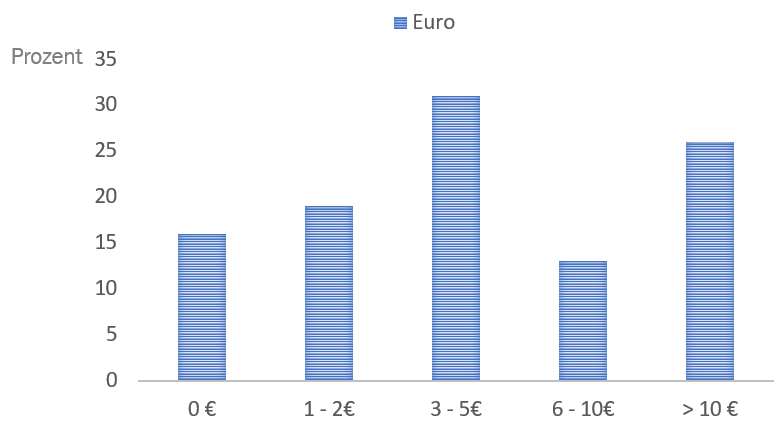
\includegraphics[width=0.7\linewidth]{Picture/umfrage_betrag}
	\caption[Zahlungsbereitschaft der Teilnehmer nach Betrag]{Zahlungsbereitschaft der Teilnehmer nach Betrag}
	\label{fig:umfrage_betrag}
\end{figure}

Den Teilnehmern ist die Privatsphäre im Bereich Banking, Haussteuerung, Handysteuerung, Soziale Netzwerke und Chatting besonders wichtig, wie in Abbildung \ref{fig:umfrage_anwendung} ersichtlich. 


\begin{figure}[h!]
	\centering
	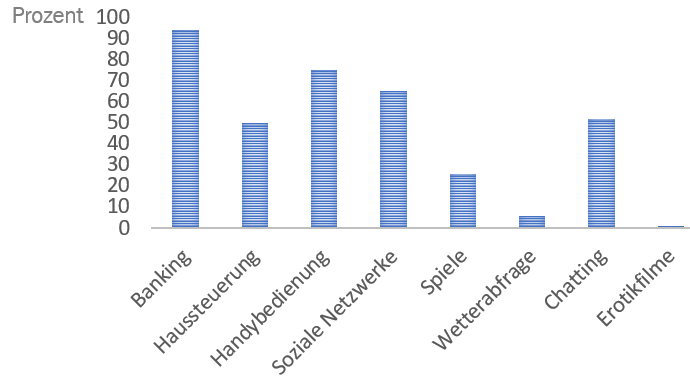
\includegraphics[width=0.7\linewidth]{Picture/umfrage_anwendung}
	\caption[Datenschutzrelevante Anwendungen der Umfrageteilnehmers]{Datenschutzrelevante Anwendungen der Umfrageteilnehmer}
	\label{fig:umfrage_anwendung}
\end{figure}

Für ein Personal Assistant Konzept, welcher Privacyaspekte des Nutzers berücksichtigt, sind folgende Schlussfolgerungen aus der Umfrage angenommen:
\begin{itemize}	
	\item Personen nutzen teilweise Sprachassistenten
	\item Die Nutzer wissen nicht, was mit ihren Daten passiert
	\item Nutzer würden für bestimmte Anwendungen Geld bezahlen, wenn diese ihre Daten schützt
	\item Datenschutz ist in den Bereichen Banking, Chatting, Haussteuerung, Social Media und Handysteuerung wichtig.
\end{itemize}
